\subsubsection{Modelo recurrente \acrshort{lstm}}

Este modelo es igual que el modelo recurrente básico pero sustituyendo la capa recurrente por una capa \acrshort{lstm} la cual es más compleja y permite que la red aprenda pueda usar mayor cantidad de información del pasado como se explicó en la sección \ref{lstm_theory}. Esta capa recurrente tiene $128$ unidades y gráficamente el modelo se puede representar de la siguiente forma:
\begin{figure}[H]
    \centering
    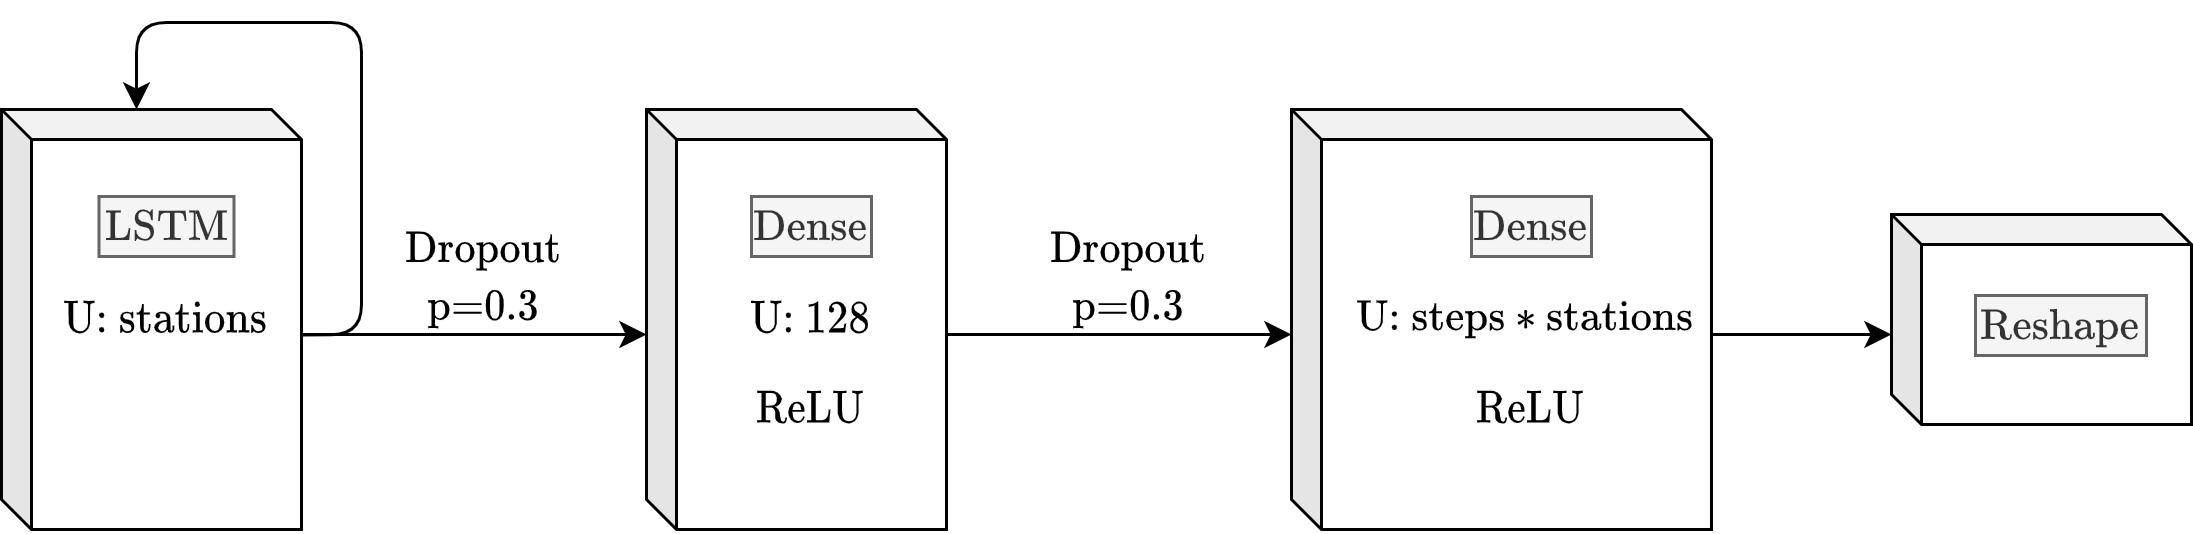
\includegraphics[width=12cm]{images/solution/models/LSTM.png}
    \caption{Modelo recurrente \acrshort{lstm}}
    \label{fig:dense-model}
\end{figure}

Como se puede observar es el mismo modelo pero sustituyendo la capa \textit{SimpleRNN} por una \acrshort{lstm}. El código de este modelo se ha definido como se muestra a continuación:
\begin{minted}[fontsize=\scriptsize]{python}
from tensorflow.keras.models import Sequential
from tensorflow.keras.layers import Reshape, Dense, Dropout, Lambda, LSTM

# `steps` is a variable which has the number of intervals to be predict
steps = 0 

# `stations` is the number of stations in the bike network
stations = 0

lstm_model = Sequential([
    # LSTM layer
    LSTM(stations, return_sequences=False),
    
    Dropout(0.3),
    Dense(128, activation="relu"),
    
    # Output layer
    Dropout(0.3),
    Dense(steps * stations, activation="relu"),
    
    # Vector to matrix
    Reshape([steps, stations])
])
\end{minted}

Los resultados del modelo se pueden ver junto al resto de resultados en la sección \ref{results}.